\chapter{Second deliverable}
\section{CAPS}
\subsection{CAPS Diagrams}
\begin{figure}[H]
\centering
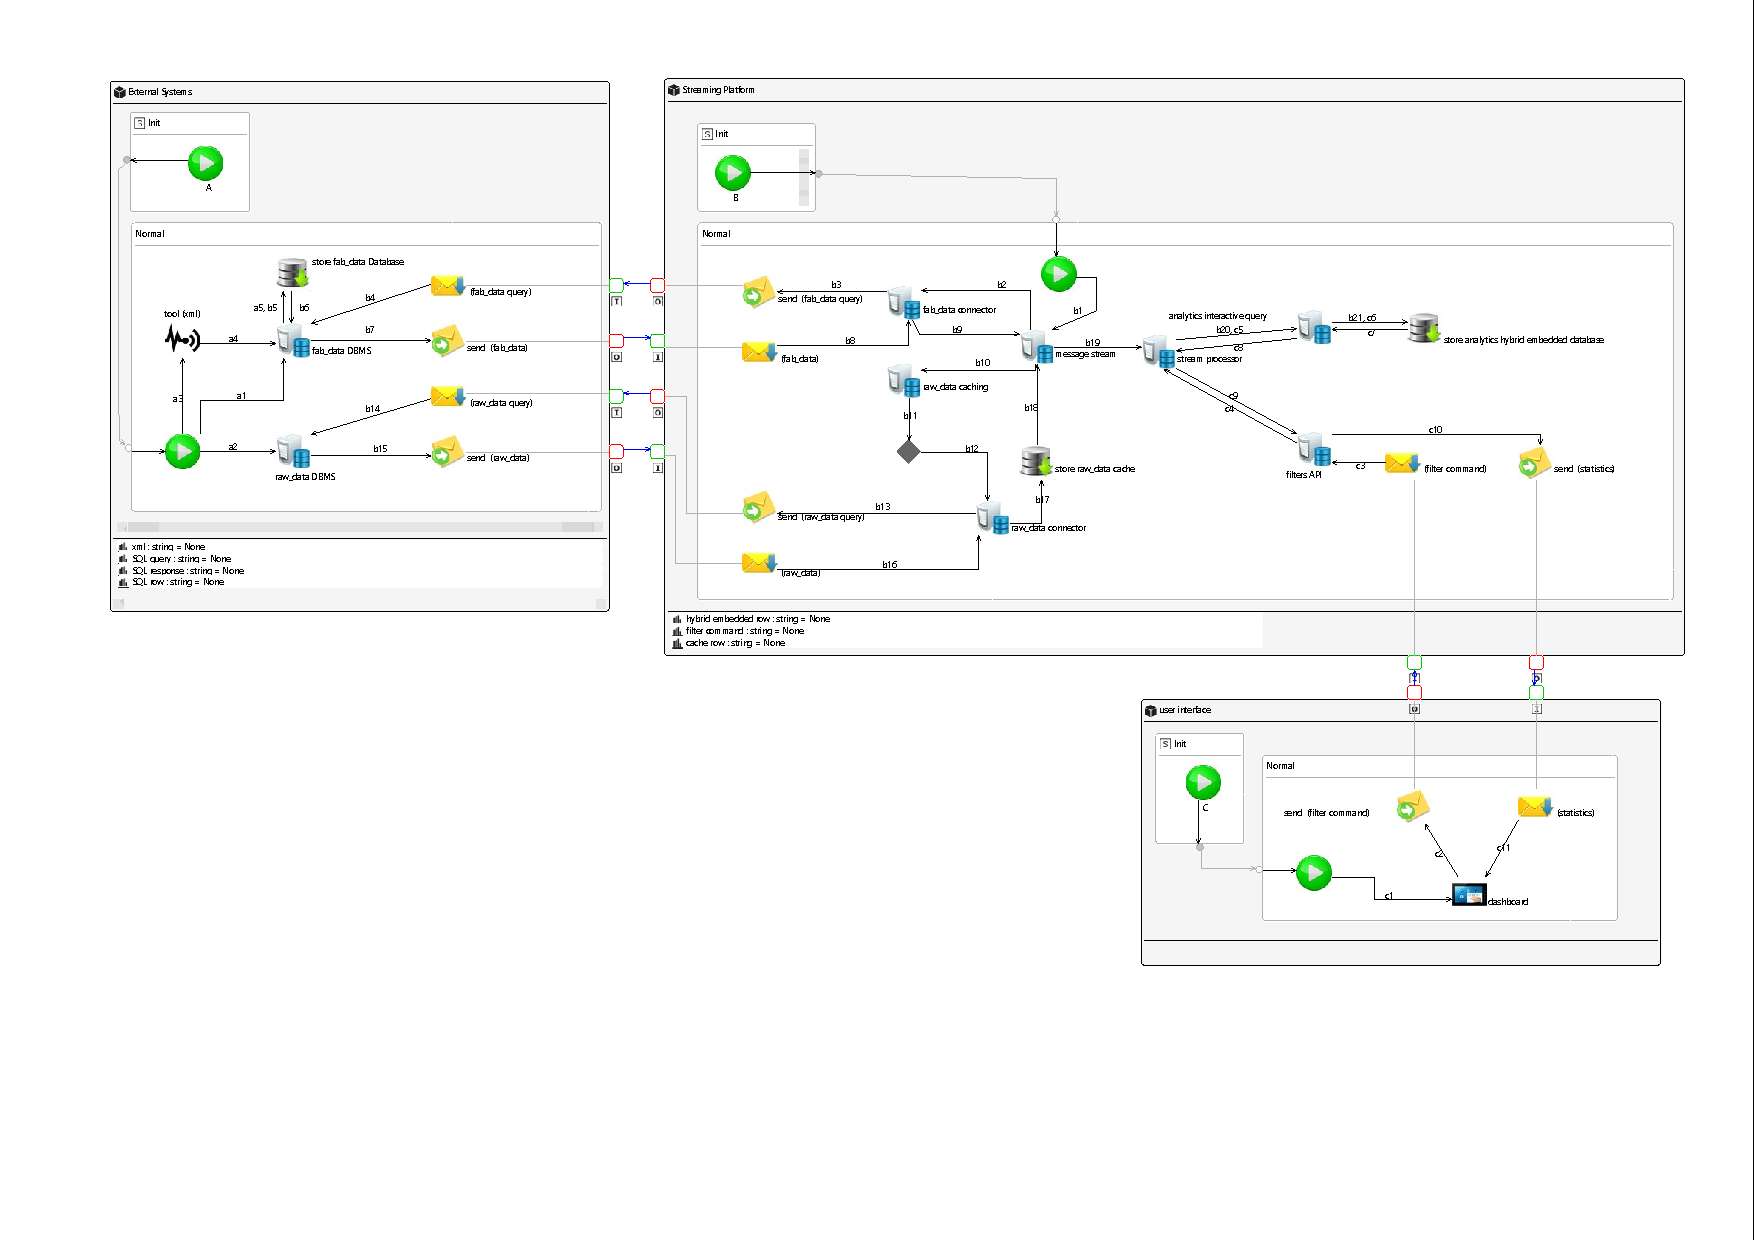
\includegraphics[trim={1.8cm 4cm 1cm 1.2cm},clip, width=\textwidth]{img/SAML.pdf}
\caption{SAML Diagram}
\end{figure}
The MEB-POC SAML Diagram source-code is downloadable from \href{https://drive.google.com/file/d/1ef9sZ7FFk_6fUsoZxO2Dyb8F9S59mnfx/view?usp=sharing}{Google Drive} and also available at \href{https://github.com/LuigiCerone/MEB-POC/tree/CAPS}{the "CAPS" branch of the project\'s github repository} (at the moment the repository is private).
\newpage
\subsection{CAPS Design Decisions}
\subsubsection{Design Decision 1}


\begin{figure}[H]
\centering
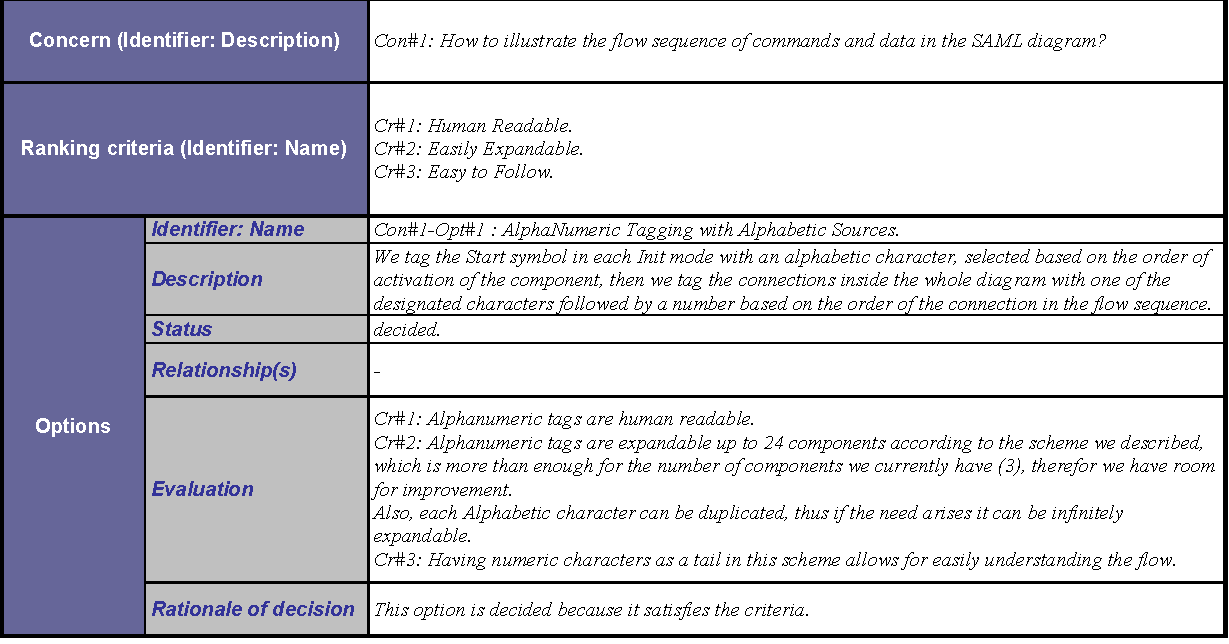
\includegraphics[width=\textwidth]{dd/DD-CAPS}
\caption{CAPS design decision}
\end{figure}

\subsubsection{Design Decision 2}
In the SAML diagram, we have decided to illustrate the tool output as XML, as indicated in the System Specification, it is therefore assumed that the fab\_data DBMS has a plugin or an extention capable of understanding that format and performing any necessary conversion of XML into a suitable format for the fab\_data database.
\newpage
\section{From architecture to code}

\subsection{Implemented service}
The system proposed in the previous chapters has been implemented in all its parts by using Kafka framework and by simulating the external databases with an ad-hoc tool developed by the team. The code for the MEB-POC system is downloadable from \href{https://drive.google.com/file/d/1CoNjQ_QpPEka4pH3k3aG3dxaqVhfUVZK/view?usp=sharing}{Google Drive} and is also available in \href{https://github.com/LuigiCerone/MEB-POC}{the "master" branch of the project\'s github repository} (at the moment the repository is private). The simulator's code is downloadable from \href{https://drive.google.com/file/d/1Qs3vJLEiLnZ-XM0G12GDj06ffdyb5ONJ/view?usp=sharing}{Google Drive} and, as above, available at \href{https://github.com/LuigiCerone/DBs\_Simulator}{github}(now the repository is private).
The language used is Java and there is an appendix chapter that tries to describe the steps needed to run the system on another laptop. \\
A short video that show the execution of the prototype is available at \\ \href{https://youtu.be/ARS0Be7CP28}{https://youtu.be/ARS0Be7CP28}. \\ 

Overall all the external dependencies of the system and the tools used by the team to develop it are:
\begin{itemize}
    \item Kafka Stream and Kafka Processor API,
    \item Jackson library for POJO serialization/deserialization,
    \item Jersey library for the RESTful interface used to implement the dashboard,
    \item MongoDB driver used to access an external backup database,
    \item Maven as dependencies manager,
    \item Git as version control manager.
\end{itemize}

The final translated information are stored both in the Kafka Stream Local State in a persistent way and also in an external MongoDB database.
The following is a diagram that represents the topics used in the system and that tries to explain the flow of information:

\begin{figure}[H]
\centering
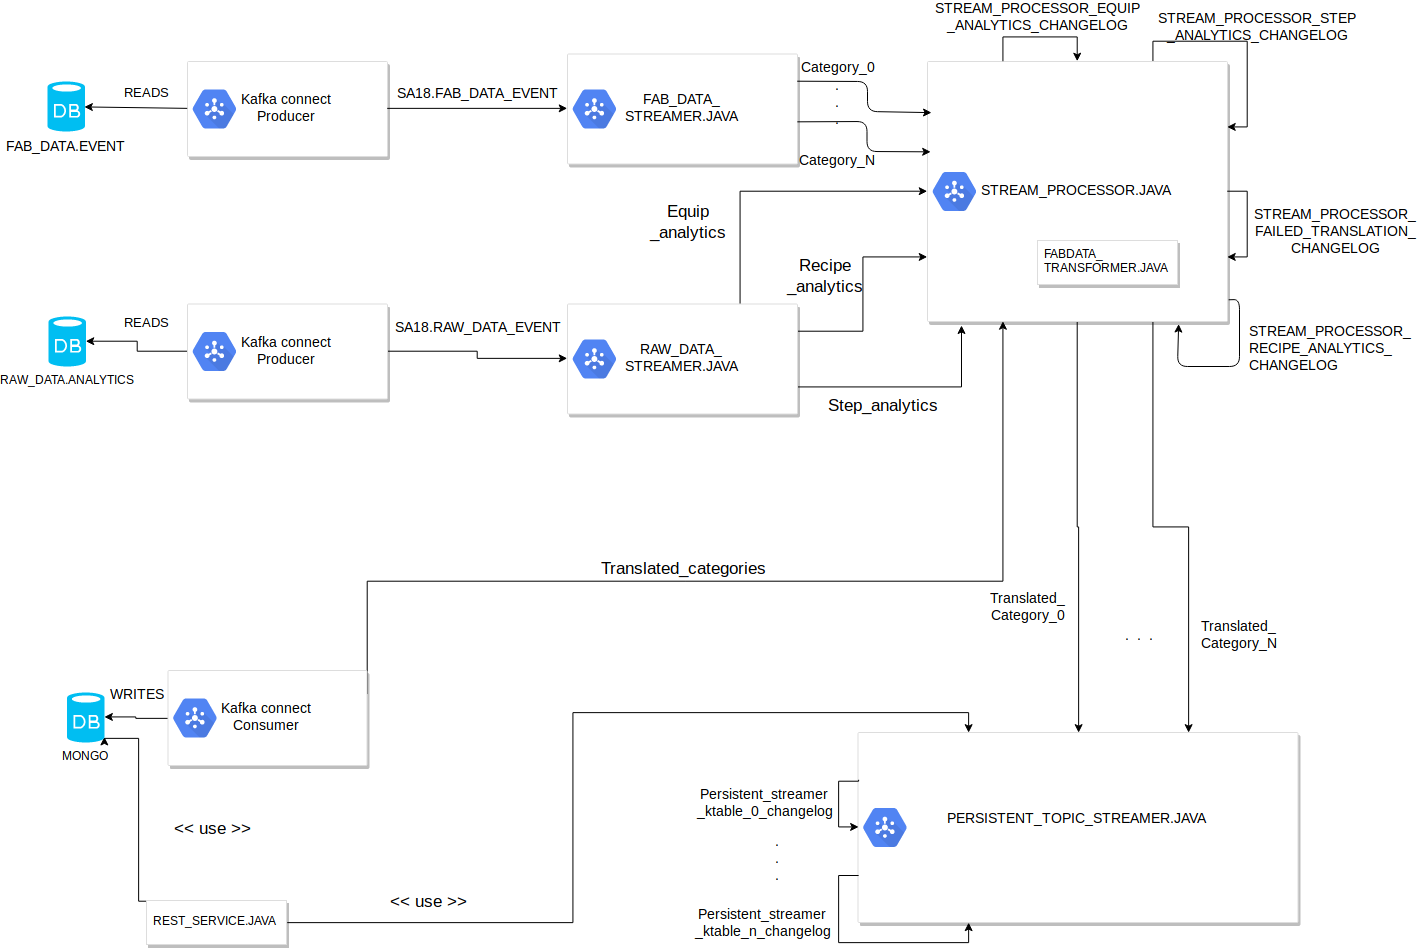
\includegraphics[width=\textwidth]{img/diagram_topics.png} \\
\caption{Used topics for the communcation}
\end{figure}


The text written above the lines represents the topic used to communicate between the classes. The topics: streamer-processor-equip\_analytics-changelog, streamer-processor-recipe\_analytics-changelog, streamer-processor-step\_analytics-changelog are \textbf{persistent} topics i.e. when the system is shut down the data they contains is not lost because it is written into the disk of the kafka's cluster computers. These topics contains the mappings used for translation in the form OID --> Translation. The topic streamer-processor-failed\_translations-changelog is another \textbf{persistent} topic where there are written the FabEvent that our system couldn't translate (major details about the translation topic is in the following section).
All the topics of the form persistent-streamer-ktable\_NUMBER-changelog are used to store the result of the translation for each category in a \textbf{permanent} way, in this way this information benefits of kafka fault tolerance and replication. Also, by using the Interactive Query API \footnote{\url{https://kafka.apache.org/10/documentation/streams/developer-guide/interactive-queries.html}}, these data could be queried with an SQL-like syntax\footnote{\url{https://www.confluent.io/product/ksql/}}.

The prototype has been implemented in package whose names respect the component diagram's one. The following is the class diagram relative to the Message Stream component:

 \begin{figure}[H]
\centering
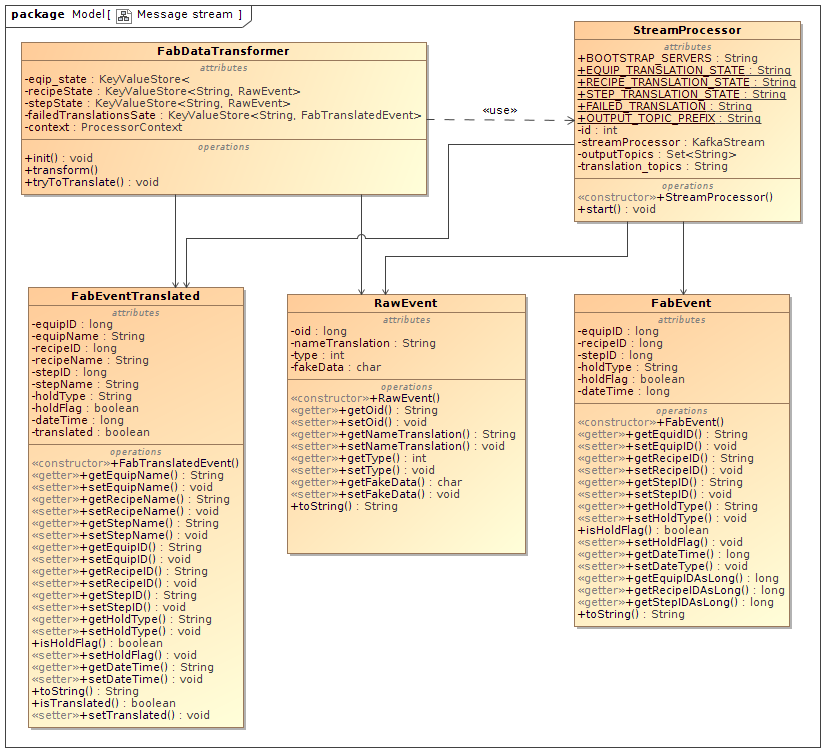
\includegraphics[width=\textwidth]{img/Class_Diagram.png} \\
\caption{Class diagram for package \textbf{message\_stream}}
\end{figure}

This package contains all the logic about the translation from a FabConnectEvent's object into a FabTranslatedEvent one. In the following section there is an activity diagram that describes the algorithm used to perform this operation.

\subsection{Translation logic}
\newpage

 \begin{figure}[H]
 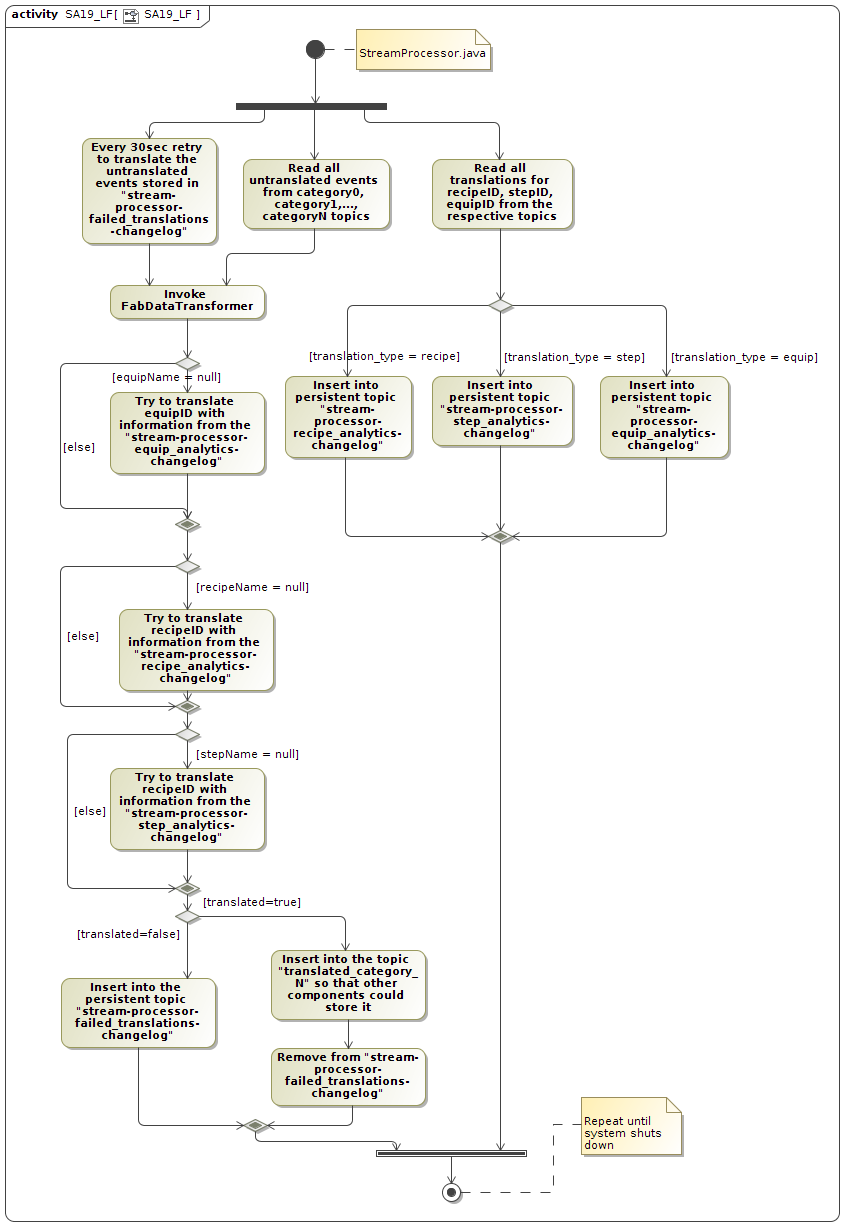
\includegraphics[width=\textwidth, scale=0.7]{img/activity.png}
\caption{Activity diagram for translation logic.}
\end{figure}

\subsection{Tests}
In the requirements section we said that our system should be albe to scale up to 160.000 msg every 30 mins. This means almost 5300 msg every minute, so one msg every 11ms.

\begin{table}[H]
\caption{Tests}
\centering
\begin{tabular}{ |c|c| } \hline
\textbf{Number of messages sent from simulator} & \textbf{Time} \\ \hline
6.600 & 75837ms $\approx 1 msg/11ms $ \\ \hline
\end{tabular}
\label{table1}
\end{table}
We did our tests on a single laptop, meaning that the pc was both running the simulator and the prototype of our system. So the kafka cluster was composed by only one pc. This means that in a production environment where there is a cluster of brokers among which the operations could be separated by using publish/subscribe architecture, our system could increase its performance. Also another thing to note about our tests is that the simulation of the external databases is computational expensive.

In order to test the size of the messages in the raw\_data database we added a fake field called fakeData used to grow the size of the message. We tried our system with it but, given the fact that the simulation requires high computational power, team thinks that the final stats could be further improved.


\section{Conclusion}

The system architecture proposed in the first chapter is based on a publish/subscribe pattern, implemented using the Kafka framework.
All the translated information are stored in the Kafka Streams local state and also in an external database (in our case a MongoDB's one).
The architecture (and so the prototype) has a series of advantages provided by the Kafka framework, such as:
\begin{itemize}
    \item If a producer loses the connection to the cluster it will wait for the connection to come back online without crashing or losing messages.
    \item If a consuming client loses the connection it will simply wait for the cluster to come back online and it will resume the consumption from where it left
    \item The information stored in the local state are replicated in the kafka cluster, in this way the final information are stored in a reliable and fault-tolerant manner.
    \item If there is a particular category in which the load of work is heavier with respect to the others, we can add more computational power to the kafka cluster thanks to its \textbf{horizontal scalability}.
    \item The components are decoupled from each other, this is a typical advantage of publish/subscribe architecture.
\end{itemize}

So, to summarize, we can say that the chosen architecture has proven us to be able to scale up to the requested messages ratio.